\section{Casi d'uso}
\begin{figure} [H]
\centering
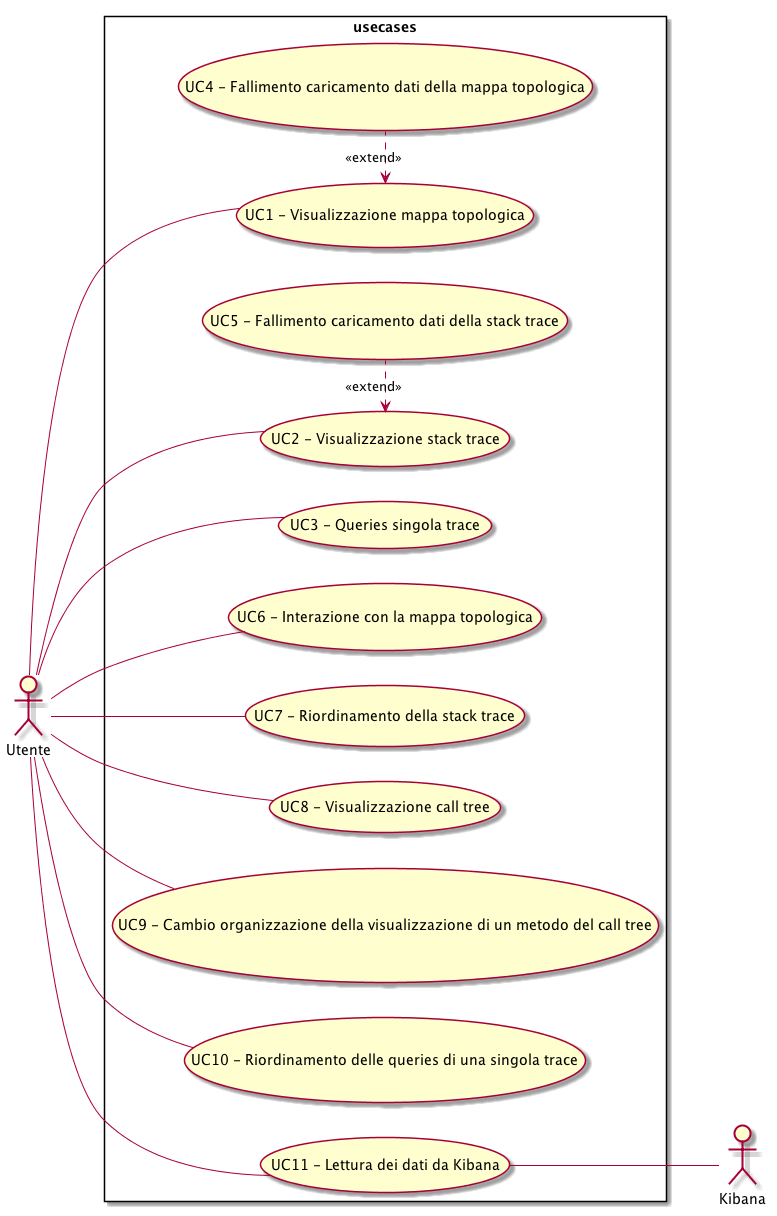
\includegraphics[scale=0.45]{./UC/UC.png}
\caption{Visualizzazione di tutti gli usecase padre}\label{}
\subsection{Caso d'uso UC1: Visualizzazione mappa topologica}
\end{figure}
\begin{figure} [H]
\centering
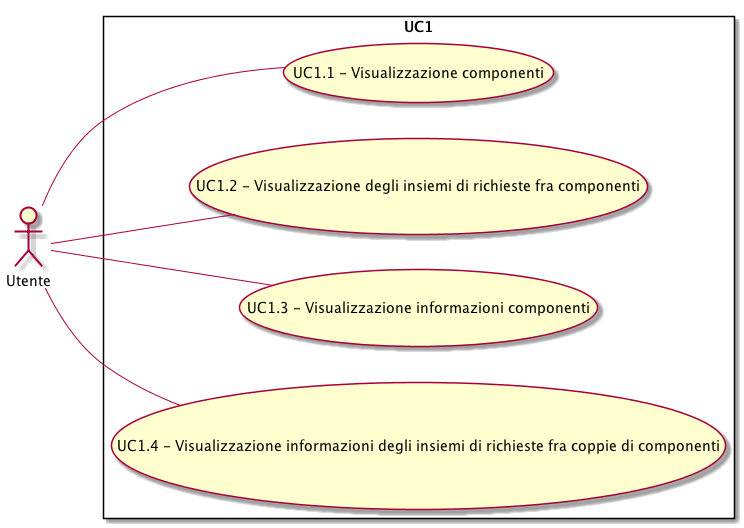
\includegraphics[scale=0.45]{./UC/UC1.png}
\caption{Visualizzazione mappa topologica}\label{}
\end{figure}
\begin{itemize}
\item \textbf{Attori}: Utente
\item \textbf{Descrizione}: L'attore intende visualizzare la mappa topologica dell'applicazione monitorata.
\item \textbf{Precondizione}: Kibana deve avere una dashboard che contenga il plugin della mappa.
\item \textbf{Flusso principale degli eventi}: L'attore richiede di visualizzare la mappa dell'applicazione monitorata, il plugin carica ed elabora i dati relativi all'applicazione monitorata, il plugin mostra la mappa topologica dell'applicazione monitorata.
\begin{itemize}
\item Visualizzazione componenti (UC1.1)
\item Visualizzazione degli insiemi di richieste fra componenti (UC1.2)
\item Visualizzazione informazioni componenti (UC1.3)
\item Visualizzazione informazioni degli insiemi di richieste fra coppie di componenti (UC1.4)
\end{itemize}
\item \textbf{Postcondizione}: Viene mostrata la mappa topologica associata all'applicazione monitorata.
\end{itemize}
\subsection{Caso d'uso UC1.1: Visualizzazione componenti}
\begin{figure} [H]
\centering
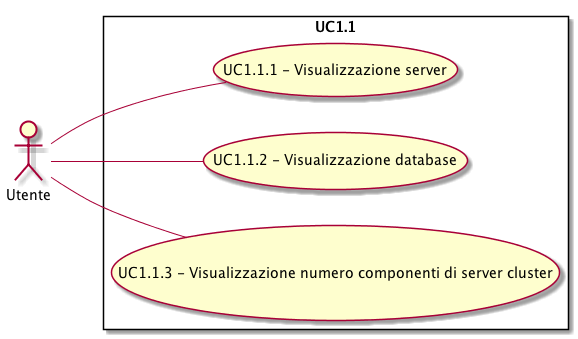
\includegraphics[scale=0.45]{./UC/UC1-1.png}
\caption{Visualizzazione componenti}\label{}
\end{figure}
\begin{itemize}
\item \textbf{Attori}: Utente
\item \textbf{Descrizione}: L'attore intende visualizzare i componenti dell'applicazione monitorata.
\item \textbf{Precondizione}: Kibana deve avere una dashboard che contenga il plugin della mappa.
\item \textbf{Flusso principale degli eventi}: L'attore intende visualizzare i componenti dell'applicazione nella mappa, quindi essi vengono disegnati all'interno di essa.
\begin{itemize}
\item Visualizzazione server (UC1.1.1)
\item Visualizzazione database (UC1.1.2)
\item Visualizzazione numero componenti di server cluster (UC1.1.3)
\end{itemize}
\item \textbf{Postcondizione}: I componenti vengono visualizzati all'interno della mappa.
\end{itemize}
\subsection{Caso d'uso UC1.1.1: Visualizzazione server}
\begin{itemize}
\item \textbf{Attori}: Utente
\item \textbf{Descrizione}: L'attore intende visualizzare nella mappa topologica i server presenti nell'applicazione monitorata.
\item \textbf{Precondizione}: Kibana deve avere una dashboard che contenga il plugin della mappa.
\item \textbf{Flusso principale degli eventi}: L'attore intende visualizzare i server presenti nell'applicazione monitorata, essi vengono quindi disegnati all'interno della mappa.
\item \textbf{Postcondizione}: Vengono mostrati i server nella  mappa topologica dell'applicazione monitorata.
\end{itemize}
\subsection{Caso d'uso UC1.1.2: Visualizzazione database}
\begin{itemize}
\item \textbf{Attori}: Utente
\item \textbf{Descrizione}: L'attore intende visualizzare nella mappa topologica i database presenti nell'applicazione monitorata.
\item \textbf{Precondizione}: Kibana deve avere una dashboard che contenga il plugin della mappa.
\item \textbf{Flusso principale degli eventi}: L'attore intende visualizzare i database presenti nell'applicazione monitorata, essi vengono quindi disegnati all'interno della mappa.
\item \textbf{Postcondizione}: Vengono mostrati i database nella mappa topologica dell'applicazione monitorata.
\end{itemize}
\subsection{Caso d'uso UC1.1.3: Visualizzazione numero componenti di server cluster}
\begin{itemize}
\item \textbf{Attori}: Utente
\item \textbf{Descrizione}: L'attore intende visualizzare nella mappa topologica, per ogni server cluster il numero di server che lo compongono.
\item \textbf{Precondizione}: Kibana deve avere una dashboard che contenga il plugin della mappa.
\item \textbf{Flusso principale degli eventi}: L'attore intende visualizzare il numero di server che compongono ciascun server cluster presente nell'applicazione monitorata, dunque per ciascuno di essi viene disegnato il numero di server di cui è composto.
\item \textbf{Postcondizione}: Per ogni server cluster presente nella mappa viene visualizzato il relativo numero di server che lo compongono.
\end{itemize}
\subsection{Caso d'uso UC1.2: Visualizzazione degli insiemi di richieste fra componenti}
\begin{figure} [H]
\centering
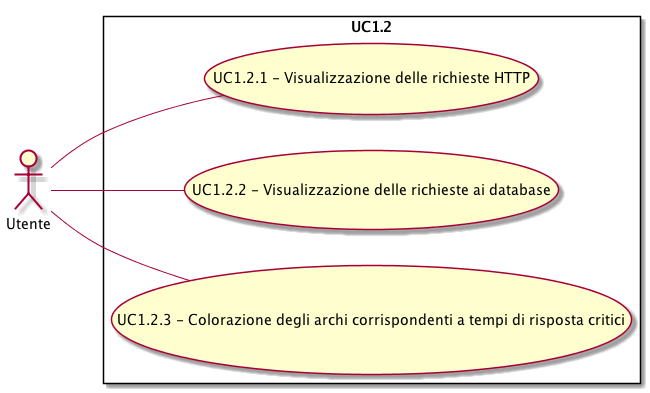
\includegraphics[scale=0.45]{./UC/UC1-2.png}
\caption{Visualizzazione degli insiemi di richieste fra componenti}\label{}
\end{figure}
\begin{itemize}
\item \textbf{Attori}: Utente
\item \textbf{Descrizione}: L'attore intende visualizzare gli insiemi di richieste fra le coppie di componenti dell'applicazione monitorata sotto forma di archi.
\item \textbf{Precondizione}: Kibana deve avere una dashboard che contenga il plugin della mappa.
\item \textbf{Flusso principale degli eventi}: L'attore intende visualizzare gli insiemi di richieste fra coppie di componenti dell'applicazione nella mappa, quindi essi vengono disegnati all'interno di essa sotto forma di archi.
\begin{itemize}
\item Visualizzazione delle richieste HTTP (UC1.2.1)
\item Visualizzazione delle richieste ai database (UC1.2.2)
\item Colorazione degli archi corrispondenti a tempi di risposta critici (UC1.2.3)
\end{itemize}
\item \textbf{Postcondizione}: Gli insiemi di richieste fra coppie di componenti vengono visualizzate all'interno della mappa sotto forma di archi.
\end{itemize}
\subsection{Caso d'uso UC1.2.1: Visualizzazione delle richieste HTTP}
\begin{itemize}
\item \textbf{Attori}: Utente
\item \textbf{Descrizione}: L'attore intende visualizzare gli insiemi di richieste HTTP fra le coppie di server dell'applicazione monitorata sotto forma di archi.
\item \textbf{Precondizione}: Kibana deve avere una dashboard che contenga il plugin della mappa.
\item \textbf{Flusso principale degli eventi}: L'attore intende visualizzare gli insiemi di richieste HTTP fra coppie di server dell'applicazione, quindi essi vengono disegnati all'interno della mappa sotto forma di archi.
\item \textbf{Postcondizione}: Gli insiemi di richieste HTTP fra coppie di componenti vengono visualizzate all'interno della mappa sotto forma di archi.
\end{itemize}
\subsection{Caso d'uso UC1.2.2: Visualizzazione delle richieste ai database}
\begin{itemize}
\item \textbf{Attori}: Utente
\item \textbf{Descrizione}: L'attore intende visualizzare gli insiemi di richieste fatte fra coppie  di server e database dell'applicazione monitorata sotto forma di archi fra i due componenti coinvolti.
\item \textbf{Precondizione}: Kibana deve avere una dashboard che contenga il plugin della mappa.
\item \textbf{Flusso principale degli eventi}: L'attore intende visualizzare gli insiemi di richieste fra coppie di server e database dell'applicazione, quindi essi vengono disegnati all'interno della mappa sotto forma di archi.
\item \textbf{Postcondizione}: Gli insiemi di richieste fra coppie di server e database vengono visualizzate all'interno della mappa sotto forma di archi.
\end{itemize}
\subsection{Caso d'uso UC1.2.3: Colorazione degli archi corrispondenti a tempi di risposta critici}
\begin{itemize}
\item \textbf{Attori}: Utente
\item \textbf{Descrizione}: L'attore intende visualizzare gli insiemi di richieste fra le coppie di componenti dell'applicazione monitorata che hanno un tempo di esecuzione medio superiore a 3 secondi come archi rossi.
\item \textbf{Precondizione}: Kibana deve avere una dashboard che contenga il plugin della mappa.
\item \textbf{Flusso principale degli eventi}: L'attore intende visualizzare gli insiemi di richieste fra coppie di componenti che hanno un tempo medio di esecuzione superiore a 3 secondi di colore rosso, quindi essi vengono disegnati all'interno della mappa sotto forma di archi di colore rosso.
\item \textbf{Postcondizione}: Gli insiemi di richieste fra coppie di componenti che hanno un tempo di esecuzione medio superiore a 3 secondi vengono visualizzate all'interno della mappa sotto forma di archi di colore rosso.
\end{itemize}
\subsection{Caso d'uso UC1.3: Visualizzazione informazioni componenti}
\begin{figure} [H]
\centering
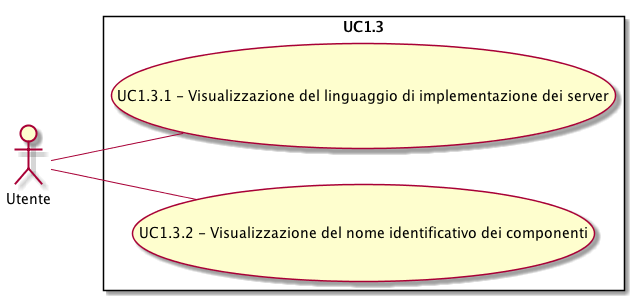
\includegraphics[scale=0.45]{./UC/UC1-3.png}
\caption{Visualizzazione informazioni componenti}\label{}
\end{figure}
\begin{itemize}
\item \textbf{Attori}: Utente
\item \textbf{Descrizione}: L'attore intende visualizzare le informazioni dei componenti dell'applicazione monitorata.
\item \textbf{Precondizione}: Kibana deve avere una dashboard che contenga il plugin della mappa.
\item \textbf{Flusso principale degli eventi}: L'attore intende visualizzare le informazioni dei componenti dell'applicazione nella mappa, quindi esse vengono rappresentate all'interno di essa accanto al relativo componente.
\begin{itemize}
\item Visualizzazione del linguaggio di implementazione dei server (UC1.3.1)
\item Visualizzazione del nome identificativo dei componenti (UC1.3.2)
\end{itemize}
\item \textbf{Postcondizione}: Le informazioni relative ad ogni componente vengono visualizzate sotto forma testuale accanto ad ognuno di essi.
\end{itemize}
\subsection{Caso d'uso UC1.3.1: Visualizzazione del linguaggio di implementazione dei server}
\begin{itemize}
\item \textbf{Attori}: Utente
\item \textbf{Descrizione}: L'attore intende visualizzare il linguaggio d'implementazione dei server.

\item \textbf{Precondizione}: Kibana deve avere una dashboard che contenga il plugin della mappa.

\item \textbf{Flusso principale degli eventi}: L'attore intende visualizzare il linguaggio di implementazione dei server presenti nella mappa topologica dell'applicazione, dunque essi vengono mostrati vicino al relativo server.
\item \textbf{Postcondizione}: Viene visualizzato il linguaggio d'implementazione dei server presenti nella mappa topologica accanto ad ognuno di essi.
\end{itemize}
\subsection{Caso d'uso UC1.3.2: Visualizzazione del nome identificativo dei componenti}
\begin{figure} [H]
\centering
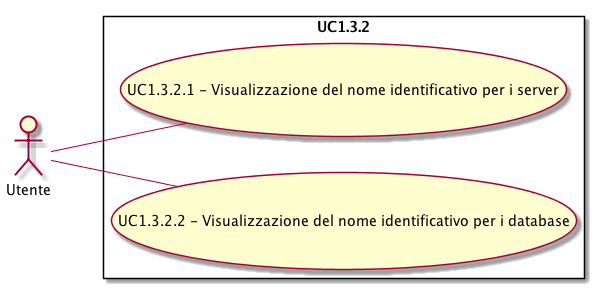
\includegraphics[scale=0.45]{./UC/UC1-3-2.png}
\caption{Visualizzazione del nome identificativo dei componenti}\label{}
\end{figure}
\begin{itemize}
\item \textbf{Attori}: Utente
\item \textbf{Descrizione}: L'attore intende visualizzare il nome di ciascun componente.
\item \textbf{Precondizione}: Kibana deve avere una dashboard che contenga il plugin della mappa.

\item \textbf{Flusso principale degli eventi}: L'attore intende visualizzare il nome identificativo di ogni componente presente nella mappa topologica che viene rappresentato accanto al componente.
\begin{itemize}
\item Visualizzazione del nome identificativo per i server (UC1.3.2.1)
\item Visualizzazione del nome identificativo per i database (UC1.3.2.2)
\end{itemize}
\item \textbf{Postcondizione}: Viene visualizzato vicino al componente il proprio nome identificativo sotto forma testuale.
\end{itemize}
\subsection{Caso d'uso UC1.3.2.1: Visualizzazione del nome identificativo per i server}
\begin{itemize}
\item \textbf{Attori}: Utente
\item \textbf{Descrizione}: L'attore intende visualizzare il nome identificativo di ciascun server presente all'interno della mappa topologica.
\item \textbf{Precondizione}: Kibana deve avere una dashboard che contenga il plugin della mappa.
\item \textbf{Flusso principale degli eventi}: L'attore intende visualizzare il nome identificativo di ogni server presente nella mappa topologica tramite l'hostname corrispondente ad ognuno di essi.
\item \textbf{Postcondizione}: Viene visualizzato vicino ad ogni server il proprio nome identificativo sotto forma testuale rappresentato dall'hostname.
\end{itemize}
\subsection{Caso d'uso UC1.3.2.2: Visualizzazione del nome identificativo per i database}
\begin{itemize}
\item \textbf{Attori}: Utente
\item \textbf{Descrizione}: L'attore intende visualizzare il nome identificativo di ciascun database presente all'interno della mappa topologica.
\item \textbf{Precondizione}: Kibana deve avere una dashboard che contenga il plugin della mappa.
\item \textbf{Flusso principale degli eventi}: L'attore intende visualizzare il nome identificativo di ogni database presente nella mappa topologica tramite il peer service corrispondente ad ognuno di essi.
\item \textbf{Postcondizione}: Viene visualizzato vicino ad ogni database il proprio nome identificativo sotto forma testuale rappresentato dal campo peer service.
\end{itemize}
\subsection{Caso d'uso UC1.4: Visualizzazione informazioni degli insiemi di richieste fra coppie di componenti}
\begin{figure} [H]
\centering
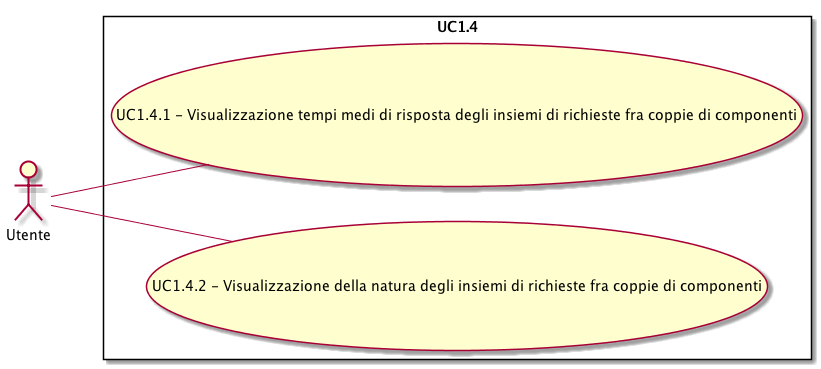
\includegraphics[scale=0.45]{./UC/UC1-4.png}
\caption{Visualizzazione informazioni degli insiemi di richieste fra coppie di componenti}\label{}
\end{figure}
\begin{itemize}
\item \textbf{Attori}: Utente
\item \textbf{Descrizione}: L'attore intende visualizzare le informazioni relative a ciascun insieme di richieste fra coppie di componenti dell'applicazione monitorata.
\item \textbf{Precondizione}: Kibana deve avere una dashboard che contenga il plugin della mappa.
\item \textbf{Flusso principale degli eventi}: L'attore intende visualizzare le informazioni relative a ciascun insieme di richieste fra coppie di componenti dell'applicazione, quindi esse vengono rappresentate all'interno della mappa sotto forma di testo vicino al relativo arco.
\begin{itemize}
\item Visualizzazione tempi medi di risposta degli insiemi di richieste fra coppie di componenti (UC1.4.1)
\item Visualizzazione della natura degli insiemi di richieste fra coppie di componenti (UC1.4.2)
\end{itemize}
\item \textbf{Postcondizione}: Le informazioni relative a ciascun insieme di richieste fra coppie di componenti vengono visualizzate all'interno della mappa.
\end{itemize}
\subsection{Caso d'uso UC1.4.1: Visualizzazione tempi medi di risposta degli insiemi di richieste fra coppie di componenti}
\begin{itemize}
\item \textbf{Attori}: Utente
\item \textbf{Descrizione}: L'attore intende visualizzare i tempi medi di risposta relativi a ciascun insieme di richieste fra coppie di componenti dell'applicazione monitorata.
\item \textbf{Precondizione}: Kibana deve avere una dashboard che contenga il plugin della mappa.
\item \textbf{Flusso principale degli eventi}: L'attore intende visualizzare i tempi medi di risposta di ciascun insieme di richieste fra coppie di componenti dell'applicazione, quindi essi vengono rappresentati all'interno di essa sotto forma di testo vicino al relativo arco.
\item \textbf{Postcondizione}: I tempi medi di risposta relativi a ciascun insieme di richieste fra coppie di componenti vengono visualizzati all'interno della mappa vicino al relativo arco che rappresenta l'insieme di richieste.
\end{itemize}
\subsection{Caso d'uso UC1.4.2: Visualizzazione della natura degli insiemi di richieste fra coppie di componenti}
\begin{figure} [H]
\centering
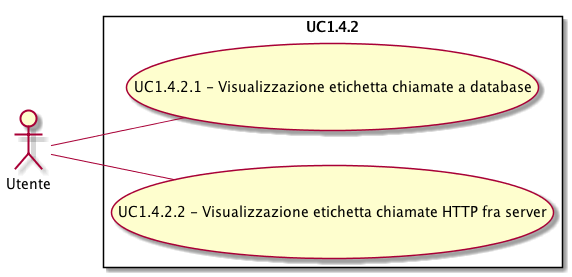
\includegraphics[scale=0.45]{./UC/UC1-4-2.png}
\caption{Visualizzazione della natura degli insiemi di richieste fra coppie di componenti}\label{}
\end{figure}
\begin{itemize}
\item \textbf{Attori}: Utente
\item \textbf{Descrizione}: L'attore intende visualizzare le nature di ciascun insieme di richieste fra coppie di componenti dell'applicazione monitorata.
\item \textbf{Precondizione}: Kibana deve avere una dashboard che contenga il plugin della mappa.
\item \textbf{Flusso principale degli eventi}: L'attore intende visualizzare le nature di ciascun insieme di richieste fra coppie di componenti dell'applicazione, quindi esse vengono rappresentate all'interno della mappa sotto forma di etichetta vicino al relativo arco.
\begin{itemize}
\item Visualizzazione etichetta chiamate a database (UC1.4.2.1)
\item Visualizzazione etichetta chiamate HTTP fra server (UC1.4.2.2)
\end{itemize}
\item \textbf{Postcondizione}: Le nature relative a ciascun insieme di richieste fra coppie di componenti vengono visualizzate all'interno della mappa vicino al relativo arco che rappresenta l'insieme di richieste.
\end{itemize}
\subsection{Caso d'uso UC1.4.2.1: Visualizzazione etichetta chiamate a database}
\begin{itemize}
\item \textbf{Attori}: Utente
\item \textbf{Descrizione}: L'attore intende visualizzare un'etichetta vicino ad ogni arco rappresentante un insieme di richieste da un server ad un database con testo "DB".
\item \textbf{Precondizione}: Kibana deve avere una dashboard che contenga il plugin della mappa.
\item \textbf{Flusso principale degli eventi}: L'attore intende visualizzare delle etichette con testo "DB" vicino ad ogni arco che rappresenti un insieme di richieste fra server e database, dunque tali etichette vengono disegnate.
\item \textbf{Postcondizione}: Vengono disegnate sulla mappa, vicino ad ogni arco che rappresenti un insieme di richieste da server a database, delle etichette con testo "DB".
\end{itemize}
\subsection{Caso d'uso UC1.4.2.2: Visualizzazione etichetta chiamate HTTP fra server}
\begin{itemize}
\item \textbf{Attori}: Utente
\item \textbf{Descrizione}: L'attore intende visualizzare un'etichetta vicino ad ogni arco rappresentante un insieme di richieste HTTP da un server ad un altro server con testo "HTTP".
\item \textbf{Precondizione}: Kibana deve avere una dashboard che contenga il plugin della mappa.
\item \textbf{Flusso principale degli eventi}: L'attore intende visualizzare delle etichette con testo "HTTP" vicino ad ogni arco che rappresenti un insieme di richieste HTTP fra server e server, dunque tali etichette vengono disegnate.
\item \textbf{Postcondizione}: Vengono disegnate sulla mappa, vicino ad ogni arco che rappresenti un insieme di richieste HTTP da server ad un altro server, delle etichette con testo "HTTP".
\end{itemize}
\subsection{Caso d'uso UC2: Visualizzazione stack trace}
\begin{figure} [H]
\centering
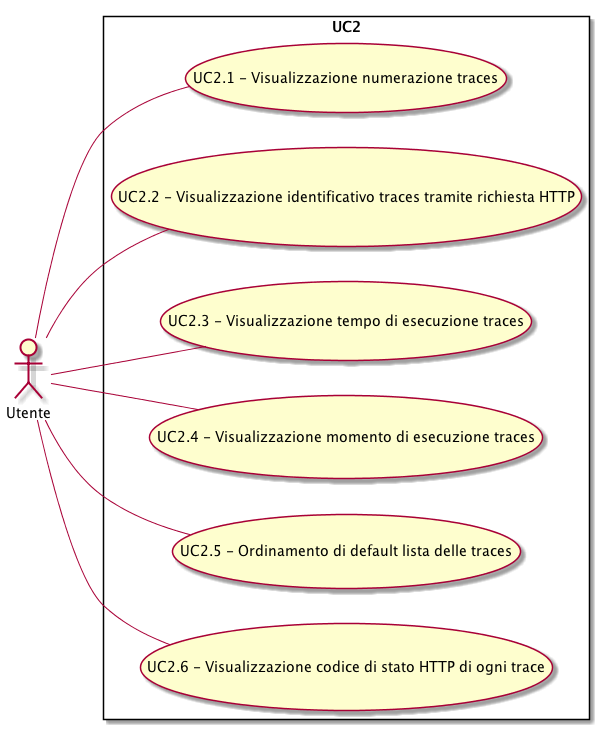
\includegraphics[scale=0.45]{./UC/UC2.png}
\caption{Visualizzazione stack trace}\label{}
\end{figure}
\begin{itemize}
\item \textbf{Attori}: Utente
\item \textbf{Descrizione}: L'attore intende visualizzare la lista delle trace dell'applicazione monitorata. 
\item \textbf{Precondizione}: Kibana deve avere una dashboard che contenga il plugin della stack trace.
\item \textbf{Flusso principale degli eventi}: L'attore intende visualizzare la lista delle trace dell'applicazione monitorata, il plugin carica ed elabora i dati relativi alle traces, dunque mostra all'attore la lista delle traces
\begin{itemize}
\item Visualizzazione numerazione traces (UC2.1)
\item Visualizzazione identificativo traces tramite richiesta HTTP (UC2.2)
\item Visualizzazione tempo di esecuzione traces (UC2.3)
\item Visualizzazione momento di esecuzione traces (UC2.4)
\item Ordinamento di default lista delle traces (UC2.5)
\item Visualizzazione codice di stato HTTP di ogni trace (UC2.6)
\end{itemize}
\item \textbf{Postcondizione}: Viene mostrato l'elenco delle traces.
\end{itemize}
\subsection{Caso d'uso UC2.1: Visualizzazione numerazione traces}
\begin{itemize}
\item \textbf{Attori}: Utente
\item \textbf{Descrizione}: L'attore intende visualizzare la lista delle traces come un elenco numerato che parta da 1.
\item \textbf{Precondizione}: Kibana deve avere una dashboard che contenga il plugin della lista delle traces.
\item \textbf{Flusso principale degli eventi}: L'attore intende visualizzare la lista delle traces come un elenco numerato, quindi vicino ad ogni trace viene disegnato un numero incrementale che parte da 1.
\item \textbf{Postcondizione}: La lista delle traces viene visualizzata come un elenco numerato.
\end{itemize}
\subsection{Caso d'uso UC2.2: Visualizzazione identificativo traces tramite richiesta HTTP}
\begin{itemize}
\item \textbf{Attori}: Utente
\item \textbf{Descrizione}: L'attore intende visualizzare le traces identificandole con la richiesta HTTP effettuata da ognuna di esse.
\item \textbf{Precondizione}: Kibana deve avere una dashboard che contenga il plugin della stack trace.
\item \textbf{Flusso principale degli eventi}: L'attore intende visualizzare la lista delle traces tramite la richiesta HTTP effettuata da ognuna di esse, che viene visualizzata in forma testuale.
\item \textbf{Postcondizione}: Ogni trace presente nella lista viene visualizzata con il proprio identificativo dato dalla richiesta HTTP effettuata.
\end{itemize}
\subsection{Caso d'uso UC2.3: Visualizzazione tempo di esecuzione traces}
\begin{itemize}
\item \textbf{Attori}: Utente
\item \textbf{Descrizione}: L'attore intende visualizzare il tempo di esecuzione di ogni trace.
\item \textbf{Precondizione}: Kibana deve avere una dashboard che contenga il plugin della stack trace.
\item \textbf{Flusso principale degli eventi}: L'attore intende visualizzare il tempo di esecuzione di ogni trace ed esso viene rappresentato sotto forma di testo.
\item \textbf{Postcondizione}: Per ogni trace presente nella lista viene visualizzato il proprio tempo di esecuzione.
\end{itemize}
\subsection{Caso d'uso UC2.4: Visualizzazione momento di esecuzione traces}
\begin{itemize}
\item \textbf{Attori}: Utente
\item \textbf{Descrizione}: L'attore intende visualizzare data e orario del momento in cui è iniziata l'esecuzione di ogni trace.
\item \textbf{Precondizione}: Kibana deve avere una dashboard che contenga il plugin della stack trace.
\item \textbf{Flusso principale degli eventi}: L'attore intende visualizzare data e orario del momento in cui è iniziata l'esecuzione di ogni trace dunque tali informazioni vengono rappresentate in maniera testuale.
\item \textbf{Postcondizione}: Vengono mostrate la data e l'orario del momento in cui è iniziata l'esecuzione di ogni trace.
\end{itemize}
\subsection{Caso d'uso UC2.5: Ordinamento di default lista delle traces}
\begin{itemize}
\item \textbf{Attori}: Utente
\item \textbf{Descrizione}: L'attore intende visualizzare la lista delle traces ordinata di default secondo un ordine cronologico decrescente del momento di esecuzione.
\item \textbf{Precondizione}: Kibana deve avere una dashboard che contenga il plugin della stack trace.
\item \textbf{Flusso principale degli eventi}: L'attore intende visualizzare la lista delle traces ordinata di default secondo un ordine cronologico decrescente del momento di esecuzione quindi queste vengono ordinate secondo questo criterio.
\item \textbf{Postcondizione}: La lista delle traces viene caricata di default in ordine cronologico decrescente del momento di esecuzione.
\end{itemize}
\subsection{Caso d'uso UC2.6: Visualizzazione codice di stato HTTP di ogni trace}
\begin{figure} [H]
\centering
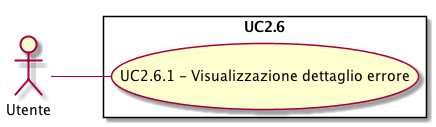
\includegraphics[scale=0.45]{./UC/UC2-6.png}
\caption{Visualizzazione codice di stato HTTP di ogni trace}\label{}
\end{figure}
\begin{itemize}
\item \textbf{Attori}: Utente
\item \textbf{Descrizione}: L'attore intende visualizzare il codice di stato HTTP associato ad ogni trace.
\item \textbf{Precondizione}: Kibana deve avere una dashboard che contenga il plugin della stack trace.
\item \textbf{Flusso principale degli eventi}: L'attore intende visualizzare il codice di stato HTTP di ogni trace ed esso viene rappresentato sotto forma di testo.
\begin{itemize}
\item Visualizzazione dettaglio errore (UC2.6.1)
\end{itemize}
\item \textbf{Postcondizione}: Per ogni trace presente nella lista viene visualizzato il proprio codice di stato HTTP.
\end{itemize}
\subsection{Caso d'uso UC2.6.1: Visualizzazione dettaglio errore}
\begin{itemize}
\item \textbf{Attori}: Utente
\item \textbf{Descrizione}: L'attore intende visualizzare il dettaglio dell'errore relativo alla richiesta HTTP associata ad una trace.
\item \textbf{Precondizione}: La richiesta HTTP fallisce con un relativo codice di stato.
\item \textbf{Flusso principale degli eventi}: L'attore intende visualizzare il dettaglio dell'errore avvenuto premendo un componente grafico associato al codice di stato HTTP.
\item \textbf{Postcondizione}: Per ogni trace la cui richiesta HTTP è fallita viene visualizzato un dettaglio dell'errore.
\end{itemize}
\subsection{Caso d'uso UC3: Queries singola trace}
\begin{figure} [H]
\centering
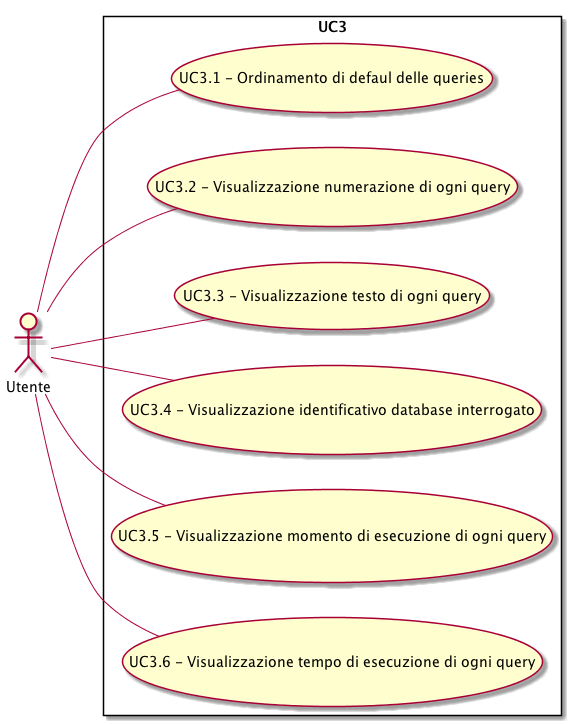
\includegraphics[scale=0.45]{./UC/UC3.png}
\caption{Queries singola trace}\label{}
\end{figure}
\begin{itemize}
\item \textbf{Attori}: Utente
\item \textbf{Descrizione}: L'attore intende visualizzare le queries eseguite in una trace.
\item \textbf{Precondizione}: Deve essere stato premuto un componente grafico adibito alla visualizzazione delle queries di una determinata trace.
\item \textbf{Flusso principale degli eventi}: L'attore richiede di visualizzare la lista delle queries eseguire da una trace quindi questa viene visualizzata.
\begin{itemize}
\item Ordinamento di defaul delle queries (UC3.1)
\item Visualizzazione numerazione di ogni query (UC3.2)
\item Visualizzazione testo di ogni query (UC3.3)
\item Visualizzazione identificativo database interrogato (UC3.4)
\item Visualizzazione momento di esecuzione di ogni query (UC3.5)
\item Visualizzazione tempo di esecuzione di ogni query (UC3.6)
\end{itemize}
\item \textbf{Scenari alternativi}: Se non sono presenti queries viene visualizzato un messaggio che informi l'attore del fatto che non sono presenti queries.
\item \textbf{Postcondizione}: Viene visualizzato l'elenco delle queries eseguite da una trace.
\end{itemize}
\subsection{Caso d'uso UC3.1: Ordinamento di defaul delle queries}
\begin{itemize}
\item \textbf{Attori}: Utente
\item \textbf{Descrizione}: L'attore intende visualizzare la lista delle queries di una singola trace ordinata di default secondo un ordine cronologico decrescente del momento di esecuzione.
\item \textbf{Precondizione}: Deve essere stato premuto un componente grafico adibito alla visualizzazione delle queries di una determinata trace.
\item \textbf{Flusso principale degli eventi}: L'attore intende visualizzare la lista delle queries di una singola trace ordinata di default secondo un ordine cronologico decrescente del momento di esecuzione quindi queste vengono ordinate in base a questo criterio.
\item \textbf{Postcondizione}: La lista delle queries di una singola trace viene caricata di default in ordine cronologico decrescente del momento di esecuzione.
\end{itemize}
\subsection{Caso d'uso UC3.2: Visualizzazione numerazione di ogni query}
\begin{itemize}
\item \textbf{Attori}: Utente
\item \textbf{Descrizione}: L'attore intende visualizzare la lista delle queries di una singola trace come un elenco numerato che parta da 1.
\item \textbf{Precondizione}: Deve essere stato premuto un componente grafico adibito alla visualizzazione delle queries di una determinata trace.
\item \textbf{Flusso principale degli eventi}: L'attore intende visualizzare la lista delle queries di una singola trace come un elenco numerato, quindi vicino ad ogni query viene disegnato un numero incrementale che parte da 1.
\item \textbf{Postcondizione}: La lista delle queries di una singola trace viene visualizzata come un elenco numerato.
\end{itemize}
\subsection{Caso d'uso UC3.3: Visualizzazione testo di ogni query}
\begin{itemize}
\item \textbf{Attori}: Utente
\item \textbf{Descrizione}: L'attore intende visualizzare il testo delle queries nella lista delle queries eseguite in una trace.
\item \textbf{Precondizione}: Deve essere stato premuto un componente grafico adibito alla visualizzazione delle queries di una determinata trace.
\item \textbf{Flusso principale degli eventi}: L'attore intende visualizzare il testo delle queries eseguite in una singola trace, dunque esso viene visualizzato.
\item \textbf{Postcondizione}: Il testo di ogni query viene visualizzato nella lista.
\end{itemize}
\subsection{Caso d'uso UC3.4: Visualizzazione identificativo database interrogato}
\begin{itemize}
\item \textbf{Attori}: Utente
\item \textbf{Descrizione}: L'attore intende visualizzare l'identificativo del database interrogato da ogni query presente nella lista queries eseguite in una trace.
\item \textbf{Precondizione}: Deve essere stato premuto un componente grafico adibito alla visualizzazione delle queries di una determinata trace.
\item \textbf{Flusso principale degli eventi}: L'attore intende visualizzare l'identificativo del database interrogato dalla query e quando la lista viene caricata nel plugin questi vengono rappresentati in forma testuale.
\item \textbf{Postcondizione}: Per ogni query nell'elenco viene visualizzato l'identificativo del database interrogato.
\end{itemize}
\subsection{Caso d'uso UC3.5: Visualizzazione momento di esecuzione di ogni query}
\begin{itemize}
\item \textbf{Attori}: Utente
\item \textbf{Descrizione}: L'attore intende visualizzare data e orario del momento in cui è iniziata l'esecuzione di ogni query.
\item \textbf{Precondizione}: Deve essere stato premuto un componente grafico adibito alla visualizzazione delle queries di una determinata trace.
\item \textbf{Flusso principale degli eventi}: L'attore intende visualizzare data e orario del momento in cui è iniziata l'esecuzione di ogni query dunque tali informazioni vengono rappresentate in maniera testuale.
\item \textbf{Postcondizione}: Vengono mostrate la data e l'orario del momento in cui è iniziata l'esecuzione di ogni query.
\end{itemize}
\subsection{Caso d'uso UC3.6: Visualizzazione tempo di esecuzione di ogni query}
\begin{itemize}
\item \textbf{Attori}: Utente
\item \textbf{Descrizione}: L'attore intende visualizzare il tempo di esecuzione di ogni query.
\item \textbf{Precondizione}: Deve essere stato premuto un componente grafico adibito alla visualizzazione delle queries di una determinata trace.
\item \textbf{Flusso principale degli eventi}: L'attore intende visualizzare il tempo di esecuzione di ogni query ed esso viene rappresentato sotto forma di testo.
\item \textbf{Postcondizione}: Per ogni query presente nella lista viene visualizzato il proprio tempo di esecuzione.
\end{itemize}
\subsection{Caso d'uso UC4: Fallimento caricamento dati della mappa topologica}
\begin{itemize}
\item \textbf{Attori}: Utente
\item \textbf{Descrizione}: I dati relativi alla mappa topologica non possono essere caricati per un errore interno.
\item \textbf{Precondizione}: Si \gl{verifica} un errore nel caricamento dei dati.
\item \textbf{Flusso principale degli eventi}: La richiesta dei dati relativi alla mappa topologica dell'applicazione monitorata non può essere soddisfatta, dunque viene visualizzato un messaggio di errore al posto della mappa.
\item \textbf{Postcondizione}: Al posto della mappa topologica viene visualizzato un messaggio di errore.
\item \textbf{Estensioni}:
\begin{itemize}
\item Visualizzazione mappa topologica (UC1)
\end{itemize}
\end{itemize}
\subsection{Caso d'uso UC5: Fallimento caricamento dati della stack trace }
\begin{itemize}
\item \textbf{Attori}: Utente
\item \textbf{Descrizione}: I dati relativi alla stack trace non possono essere caricati per un errore interno.
\item \textbf{Precondizione}: Si verifica un errore nel caricamento dei dati.
\item \textbf{Flusso principale degli eventi}: La richiesta dei dati relativi alla stack trace dell'applicazione monitorata non può essere soddisfatta, dunque viene visualizzato un messaggio di errore al posto della stack trace.
\item \textbf{Postcondizione}: Al posto della stack trace viene visualizzato un messaggio di errore.
\item \textbf{Estensioni}:
\begin{itemize}
\item Visualizzazione stack trace (UC2)
\end{itemize}
\end{itemize}
\subsection{Caso d'uso UC6: Interazione con la mappa topologica}
\begin{figure} [H]
\centering
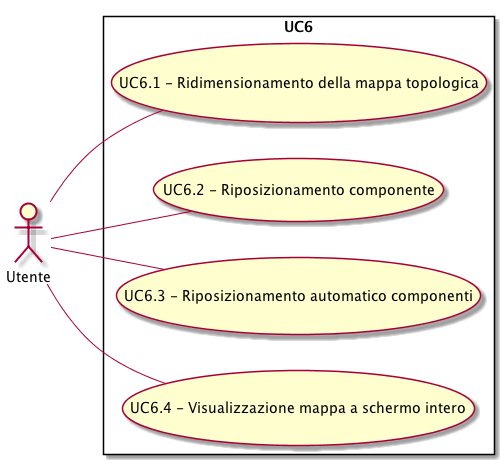
\includegraphics[scale=0.45]{./UC/UC6.png}
\caption{Interazione con la mappa topologica}\label{}
\end{figure}
\begin{itemize}
\item \textbf{Attori}: Utente
\item \textbf{Descrizione}: L'attore intende manipolare la visualizzazione della mappa topologica.
\item \textbf{Precondizione}: Deve essere visualizzata la mappa topologica dell'applicazione monitorata.
\item \textbf{Flusso principale degli eventi}: L'attore interagisce con le componenti grafiche dedicate alla manipolazione della mappa topologica e ne modifica la rappresentazione.
\begin{itemize}
\item Ridimensionamento della mappa topologica (UC6.1)
\item Riposizionamento componente (UC6.2)
\item Riposizionamento automatico componenti (UC6.3)
\item Visualizzazione mappa a schermo intero (UC6.4)
\end{itemize}
\item \textbf{Postcondizione}: La visualizzazione della mappa topologica risulta modificata come nelle intenzioni dell'attore.
\end{itemize}
\subsection{Caso d'uso UC6.1: Ridimensionamento della mappa topologica}
\begin{figure} [H]
\centering
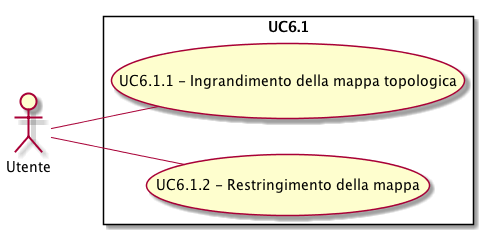
\includegraphics[scale=0.45]{./UC/UC6-1.png}
\caption{Ridimensionamento della mappa topologica}\label{}
\end{figure}
\begin{itemize}
\item \textbf{Attori}: Utente
\item \textbf{Descrizione}: L'attore intende eseguire un ridimensionamento della mappa topologica. 
\item \textbf{Precondizione}: Deve essere stato caricato il plugin della mappa topologica.
\item \textbf{Flusso principale degli eventi}: L'attore interagisce con un componente grafico che permetta il ridimensionamento della mappa, quindi essa viene ridimensionata.
\begin{itemize}
\item Ingrandimento della mappa topologica (UC6.1.1)
\item Restringimento della mappa (UC6.1.2)
\end{itemize}
\item \textbf{Scenari alternativi}: La mappa ha raggiunto dei limiti per il ridimensionamento non può essere ridimensionata.
\item \textbf{Postcondizione}: La mappa topologica viene ridimensionata. 
\end{itemize}
\subsection{Caso d'uso UC6.1.1: Ingrandimento della mappa topologica}
\begin{itemize}
\item \textbf{Attori}: Utente
\item \textbf{Descrizione}: L'attore intende ingrandire la rappresentazione grafica della mappa.
\item \textbf{Precondizione}: Deve essere stato caricato il plugin della mappa topologica dell'applicazione.
\item \textbf{Flusso principale degli eventi}: L'attore preme un componente grafico che permetta l'ingrandimento della mappa. La mappa viene quindi ingrandita.
\item \textbf{Scenari alternativi}: Se è stato raggiunto il limite massimo di ingrandimento consentito la mappa non viene ingrandita.
\item \textbf{Postcondizione}: La mappa viene ingrandita.
\end{itemize}
\subsection{Caso d'uso UC6.1.2: Restringimento della mappa}
\begin{itemize}
\item \textbf{Attori}: Utente
\item \textbf{Descrizione}: L'attore intende restringere la rappresentazione grafica della mappa.
\item \textbf{Precondizione}: Deve essere stato caricato il plugin della mappa topologica dell'applicazione.
\item \textbf{Flusso principale degli eventi}: L'attore preme un componente grafico che permetta la restrizione della mappa topologica, la rappresentazione della mappa viene ristretta.
\item \textbf{Scenari alternativi}: Se è stato raggiunto il limite massimo di restrizione consentita e la mappa non viene ristretta.
\item \textbf{Postcondizione}: La rappresentazione della mappa viene ristretta.
\end{itemize}
\subsection{Caso d'uso UC6.2: Riposizionamento componente}
\begin{itemize}
\item \textbf{Attori}: Utente
\item \textbf{Descrizione}: L'attore intende spostare un componente all'interno della mappa topologica dell'applicazione monitorata.
\item \textbf{Precondizione}: Deve essere stato caricato da Kibana il plugin della mappa topologica dell'applicazione.
\item \textbf{Flusso principale degli eventi}: L'attore trascina un componente della mappa topologica con il puntatore
Il componente trascinato viene riposizionato
\item \textbf{Postcondizione}: Il componente trascinato viene riposizionato.
\end{itemize}
\subsection{Caso d'uso UC6.3: Riposizionamento automatico componenti}
\begin{itemize}
\item \textbf{Attori}: Utente
\item \textbf{Descrizione}: L'attore intende riposizionare tutti i componenti della mappa topologica dell'applicazione monitorata in modo automatico.
\item \textbf{Precondizione}: Deve essere stato caricato da Kibana il plugin della mappa topologica dell'applicazione e qualche componente deve essere già stato riposizionato.
\item \textbf{Flusso principale degli eventi}: L'attore preme un  componente grafico che avvii il riposizionamento delle componenti 
Le componenti che sono state spostate vengono riposizionate nella loro posizione iniziale
\item \textbf{Postcondizione}: Tutti i componenti della mappa si trovano nella posizione iniziale in cui è stata caricata la mappa. 
\end{itemize}
\subsection{Caso d'uso UC6.4: Visualizzazione mappa a schermo intero}
\begin{itemize}
\item \textbf{Attori}: Utente
\item \textbf{Descrizione}: L'attore intende visualizzare la mappa a schemo intero.
\item \textbf{Precondizione}: Deve essere stata caricata la mappa topologica dell'applicazione monitorata.
\item \textbf{Flusso principale degli eventi}: L'attore preme sul componente grafico dedicato all'attivazione della modalità a schermo interro ed essa viene visualizzata  schermo intero.
\item \textbf{Postcondizione}: La mappa topologica viene visualizzata a schermo intero.
\end{itemize}
\subsection{Caso d'uso UC7: Riordinamento della stack trace.}
\begin{figure} [H]
\centering
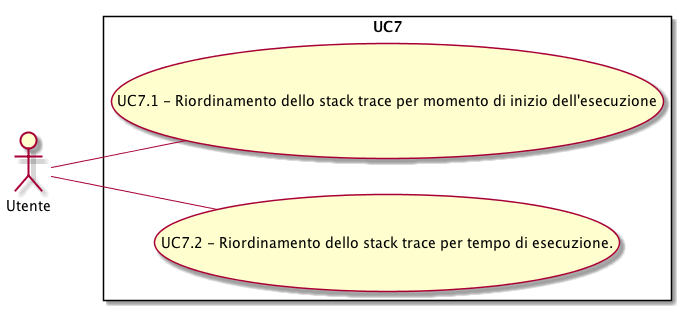
\includegraphics[scale=0.45]{./UC/UC7.png}
\caption{Riordinamento della stack trace.}\label{}
\end{figure}
\begin{itemize}
\item \textbf{Attori}: Utente
\item \textbf{Descrizione}: L'attore intende manipolare l'ordinamento dello stack trace.

\item \textbf{Precondizione}: Deve essere stata visualizzata all'interno del plugin la stack trace.

\item \textbf{Flusso principale degli eventi}: L'attore intende riordinare la stack trace e questa viene riordinata.
\begin{itemize}
\item Riordinamento dello stack trace per momento di inizio dell'esecuzione (UC7.1)
\item Riordinamento dello stack trace per tempo di esecuzione (UC7.2)
\end{itemize}
\item \textbf{Postcondizione}: La stack trace viene riordinata. 
\end{itemize}
\subsection{Caso d'uso UC7.1: Riordinamento dello stack trace per momento di inizio dell'esecuzione}
\begin{figure} [H]
\centering
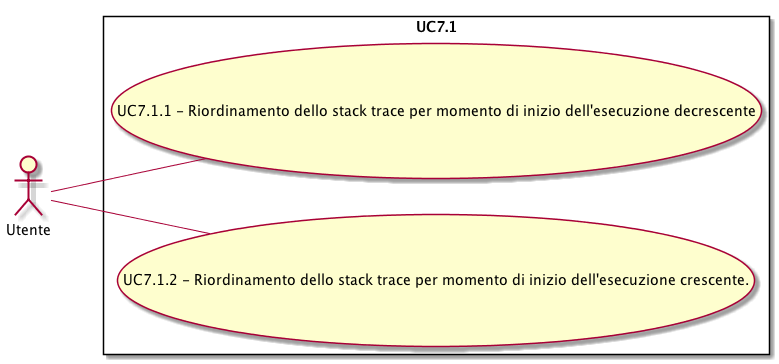
\includegraphics[scale=0.45]{./UC/UC7-1.png}
\caption{Riordinamento dello stack trace per momento di inizio dell'esecuzione}\label{}
\end{figure}
\begin{itemize}
\item \textbf{Attori}: Utente
\item \textbf{Descrizione}: L'attore vuole riordinare la lista delle traces in base al momento di inizio dell'esecuzione.
\item \textbf{Precondizione}: Deve essere stata visualizzata all'interno del plugin la stack trace.
\item \textbf{Flusso principale degli eventi}: L'attore vuole riordinare la stack trace in base al momento di inizio dell'esecuzione e questo avviene in seguito all'interazione con un componente grafico.
\begin{itemize}
\item Riordinamento dello stack trace per momento di inizio dell'esecuzione decrescente (UC7.1.1)
\item Riordinamento dello stack trace per momento di inizio dell'esecuzione crescente. (UC7.1.2)
\end{itemize}
\item \textbf{Postcondizione}: La stack trace viene riordinata in base al momento di inizio dell'esecuzione.
\end{itemize}
\subsection{Caso d'uso UC7.1.1: Riordinamento dello stack trace per momento di inizio dell'esecuzione decrescente}
\begin{itemize}
\item \textbf{Attori}: Utente
\item \textbf{Descrizione}: L'attore vuole riordinare la lista delle traces in base al momento di inizio dell'esecuzione decrescente.
\item \textbf{Precondizione}: Deve essere stata visualizzata all'interno del plugin la stack trace.
\item \textbf{Flusso principale degli eventi}: L'attore vuole riordinare la stack trace in base al momento di inizio dell'esecuzione decrescente e questo avviene in seguito all'interazione con un componente grafico.
\item \textbf{Postcondizione}: La stack trace viene riordinata in base al momento di inizio dell'esecuzione decrescente.
\end{itemize}
\subsection{Caso d'uso UC7.1.2: Riordinamento dello stack trace per momento di inizio dell'esecuzione crescente.}
\begin{itemize}
\item \textbf{Attori}: Utente
\item \textbf{Descrizione}: L'attore vuole riordinare la lista delle traces in base al momento di inizio dell'esecuzione crescente.
\item \textbf{Precondizione}: Deve essere stata visualizzata all'interno del plugin la stack trace.
\item \textbf{Flusso principale degli eventi}: L'attore vuole riordinare la stack trace in base al momento di inizio dell'esecuzione decrescente e questo avviene in seguito all'interazione con un componente grafico.
\item \textbf{Postcondizione}: La stack trace viene riordinata in base al momento di inizio dell'esecuzione crescente
\end{itemize}
\subsection{Caso d'uso UC7.2: Riordinamento dello stack trace per tempo di esecuzione}
\begin{figure} [H]
\centering
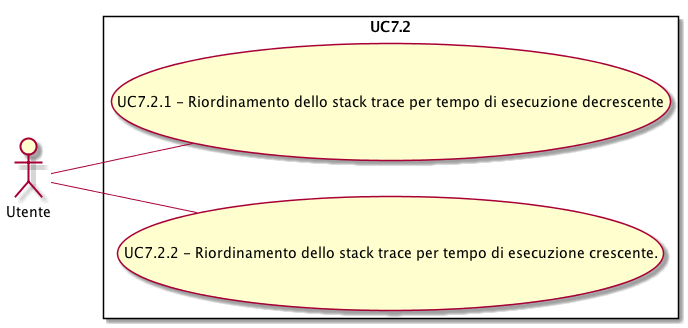
\includegraphics[scale=0.45]{./UC/UC7-2.png}
\caption{Riordinamento dello stack trace per tempo di esecuzione}\label{}
\end{figure}
\begin{itemize}
\item \textbf{Attori}: Utente
\item \textbf{Descrizione}: L'attore vuole riordinare la lista delle trace in base al tempo di esecuzione.
\item \textbf{Precondizione}: Deve essere stata visualizzata all'interno del plugin la stack trace.
\item \textbf{Flusso principale degli eventi}: L'attore vuole riordinare la stack trace in base al tempo di esecuzione e questo avviene in seguito all'interazione con un componente grafico.
\begin{itemize}
\item Riordinamento dello stack trace per tempo di esecuzione decrescente (UC7.2.1)
\item Riordinamento dello stack trace per tempo di esecuzione crescente (UC7.2.2)
\end{itemize}
\item \textbf{Postcondizione}: La stack trace viene riordinata in base al tempo di esecuzione.
\end{itemize}
\subsection{Caso d'uso UC7.2.1: Riordinamento dello stack trace per tempo di esecuzione decrescente}
\begin{itemize}
\item \textbf{Attori}: Utente
\item \textbf{Descrizione}: L'attore vuole riordinare la lista delle trace in base al tempo di esecuzione decrescente.
\item \textbf{Precondizione}: Deve essere stata visualizzata all'interno del plugin la stack trace.
\item \textbf{Flusso principale degli eventi}: L'attore vuole riordinare la stack trace in base al tempo di esecuzione decrescente e questo avviene in seguito all'interazione con un componente grafico.
\item \textbf{Postcondizione}: La stack trace viene riordinata in base al tempo di esecuzione decrescente.
\end{itemize}
\subsection{Caso d'uso UC7.2.2: Riordinamento dello stack trace per tempo di esecuzione crescente}
\begin{itemize}
\item \textbf{Attori}: Utente
\item \textbf{Descrizione}: L'attore vuole riordinare lo stack trace per tempo di esecuzione crescente.
\item \textbf{Precondizione}: Deve essere stata visualizzata all'interno del plugin la stack trace.
\item \textbf{Flusso principale degli eventi}: L'attore vuole riordinare la stack trace in base al tempo di esecuzione crescente e questo avviene in seguito all'interazione con un componente grafico.
\item \textbf{Postcondizione}: La stack trace viene riordinata in base al tempo di esecuzione crescente.
\end{itemize}
\subsection{Caso d'uso UC8: Visualizzazione call tree}
\begin{figure} [H]
\centering

\includegraphics[scale=0.45]{./UC/UC8.png}
\caption{Visualizzazione call tree}\label{}
\end{figure}
\begin{itemize}
\item \textbf{Attori}: Utente
\item \textbf{Descrizione}: L'attore intende visualizzare il call tree di una trace selezionata.
\item \textbf{Precondizione}: Deve essere stato premuto un componente grafico adibito alla visualizzazione del call tree di una determinata trace.
\item \textbf{Flusso principale degli eventi}: L'attore intende visualizzare il call tree di una determinata trace, quindi preme un componente grafico associato alla trace che ne determina la visualizzazione.
\begin{itemize}
\item Visualizzazione nome metodi (UC8.1)
\item Visualizzazione self execution time (UC8.2)
\item Visualizzazione total execution time (UC8.3)
\item Indentazione sottochiamate (UC8.4)
\item Visualizzazione di default call tree (UC8.5)
\item Visualizzazione queries di ogni metodo (UC8.6)
\end{itemize}
\item \textbf{Postcondizione}: Viene visualizzato il call tree della trace selezionata.
\end{itemize}
\subsection{Caso d'uso UC8.1: Visualizzazione nome metodi}
\begin{itemize}
\item \textbf{Attori}: Utente
\item \textbf{Descrizione}: L'attore intende visualizzare il nome di ogni metodo presente nel call tree.
\item \textbf{Precondizione}: Deve essere stato caricato il call tree di una determinata trace.
\item \textbf{Flusso principale degli eventi}: L'attore intende visualizzare il nome di ogni metodo presente nel call tree ed esso viene visualizzato forma testuale.
\item \textbf{Postcondizione}: Per ogni metodo del call tree ne viene visualizzato il nome.
\end{itemize}
\subsection{Caso d'uso UC8.2: Visualizzazione self execution time}
\begin{itemize}
\item \textbf{Attori}: Utente
\item \textbf{Descrizione}: L'attore intende visualizzare il self execution time di ogni metodo presente nel call tree.
\item \textbf{Precondizione}: Deve essere stato caricato il call tree di una determinata trace.
\item \textbf{Flusso principale degli eventi}: L'attore intende visualizzare il self execution time di ogni metodo presente nel call tree ed esso viene visualizzato in forma testuale.
\item \textbf{Postcondizione}: Per ogni metodo del call tree ne viene visualizzato il self execution time.
\end{itemize}
\subsection{Caso d'uso UC8.3: Visualizzazione total execution time}
\begin{itemize}
\item \textbf{Attori}: Utente
\item \textbf{Descrizione}: L'attore intende visualizzare il total execution time di ogni metodo presente nel call tree.
\item \textbf{Precondizione}: Deve essere stato caricato il call tree di una determinata trace.
\item \textbf{Flusso principale degli eventi}: L'attore intende visualizzare il total execution time di ogni metodo presente nel call tree ed esso viene visualizzato in forma testuale.
\item \textbf{Postcondizione}: Per ogni metodo del call tree ne viene visualizzato il total execution time.
\end{itemize}
\subsection{Caso d'uso UC8.4: Indentazione sottochiamate}
\begin{itemize}
\item \textbf{Attori}: Utente
\item \textbf{Descrizione}: L'attore intende visualizzare le sottochiamate nel call tree con indentazione incrementale per visualizzare esplicitamente le relazioni di annidamento.
\item \textbf{Precondizione}: Deve essere stato caricato il call tree di una determinata trace.
\item \textbf{Flusso principale degli eventi}: L'attore intende visualizzare il call tree con esplicite relazioni di annidamento incrementale e questo accade attraverso l'indentazione delle sottochiamate.

\item \textbf{Postcondizione}: I metodi del call tree vengono visualizzati con intestazione per esplicitare le relazioni di annidamento.
\end{itemize}
\subsection{Caso d'uso UC8.5: Visualizzazione di default call tree}
\begin{itemize}
\item \textbf{Attori}: Utente
\item \textbf{Descrizione}: L'attore intende visualizzare di default il call tree in maniera espansa.
\item \textbf{Precondizione}: Deve essere stato caricato il call tree di una determinata trace.
\item \textbf{Flusso principale degli eventi}: L'attore intende visualizzare di default il call tree in maniera espansa, quindi vengono visualizzate tutte le sottochiamate di ogni metodo.
\item \textbf{Postcondizione}: Il call tree viene visualizzato di default in maniera espansa.
\end{itemize}
\subsection{Caso d'uso UC8.6: Visualizzazione queries di ogni metodo}
\begin{itemize}
\item \textbf{Attori}: Utente
\item \textbf{Descrizione}: L'attore intende visualizzare le queries effettuate da ogni metodo del call tree.
\item \textbf{Precondizione}: Deve essere stato caricato il call tree di una determinata trace.
\item \textbf{Flusso principale degli eventi}: Per ogni metodo del call tree l'attore intende visualizzare le queries effettuate da esso, quindi ogni query viene visualizzata sotto il metodo che la ha eseguita.
\item \textbf{Postcondizione}: Per ogni metodo del call tree vengono visualizzate le queries da esso effettuate.
\end{itemize}
\subsection{Caso d'uso UC9: Cambio organizzazione della visualizzazione di un metodo del call tree}
\begin{figure} [H]
\centering
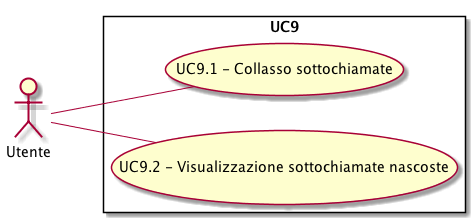
\includegraphics[scale=0.45]{./UC/UC9.png}
\caption{Cambio organizzazione della visualizzazione di un metodo del call tree}\label{}
\end{figure}
\begin{itemize}
\item \textbf{Attori}: Utente
\item \textbf{Descrizione}: L'attore intende cambiare l'organizzazione della visualizzazione di un metodo e dei propri sottometodi attraverso dei componenti grafici.
\item \textbf{Precondizione}: Deve essere stato caricato il call tree di una determinata trace.
\item \textbf{Flusso principale degli eventi}: L'attore intende cambiare l'organizzazione della visualizzazione di un metodo del call tree, quindi preme un componente grafico che permette questo.
\begin{itemize}
\item Collasso sottochiamate (UC9.1)
\item Visualizzazione sottochiamate nascoste (UC9.2)
\end{itemize}
\item \textbf{Postcondizione}: La visualizzazione di un metodo e dei suoi sottometodi viene cambiata.
\end{itemize}
\subsection{Caso d'uso UC9.1: Collasso sottochiamate}
\begin{itemize}
\item \textbf{Attori}: Utente
\item \textbf{Descrizione}: L'attore intende nascondere la lista delle sottochiamate eseguite da una singola chiamata all'interno del call tree.
\item \textbf{Precondizione}: Il call tree di una trace deve essere stato visualizzato.
\item \textbf{Flusso principale degli eventi}: L'attore clicca su un pulsante corrispondente alla chiamata della quale vuole nascondere le sottochiamate
Le sottochiamate vengono nascoste
\item \textbf{Postcondizione}: Tutte le chiamate eseguite dalla singola chiamata vengono nascoste.
\end{itemize}
\subsection{Caso d'uso UC9.2: Visualizzazione sottochiamate nascoste}
\begin{itemize}
\item \textbf{Attori}: Utente
\item \textbf{Descrizione}: L'attore intende mostrare le sottochiamate nascoste di una specifica chiamata nel call tree
\item \textbf{Precondizione}: Devono essere state nascoste le sottochiamate
\item \textbf{Flusso principale degli eventi}: L'attore clicca su un pulsante corrispondente alla chiamata della quale vuole mostrare le sottochiamate
Le sottochiamate vengono mostrate
\item \textbf{Postcondizione}: Vengono mostrate le sottochiamate di una chiamata
\end{itemize}
\subsection{Caso d'uso UC10: Riordinamento delle queries di una singola trace}
\begin{figure} [H]
\centering
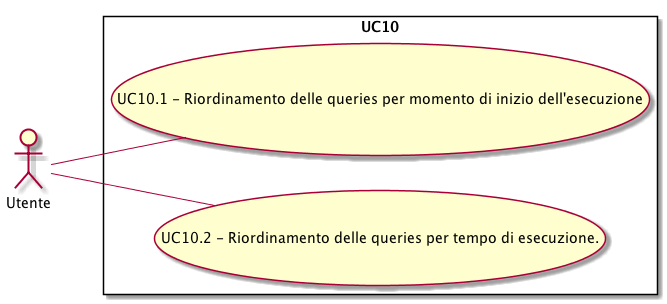
\includegraphics[scale=0.45]{./UC/UC10.png}
\caption{Riordinamento delle queries di una singola trace}\label{}
\end{figure}
\begin{itemize}
\item \textbf{Attori}: Utente
\item \textbf{Descrizione}: L'attore intende manipolare l'ordinamento delle queries di una singola trace.
\item \textbf{Precondizione}: Deve essere stata visualizzata la lista di queries di una singola trace.
\item \textbf{Flusso principale degli eventi}: L'attore intende riordinare le queries di una singola trace e queste viene riordinata.
\begin{itemize}
\item Riordinamento delle queries per momento di inizio dell'esecuzione (UC10.1)
\item Riordinamento delle queries per tempo di esecuzione (UC10.2)
\end{itemize}
\item \textbf{Postcondizione}: La lista di queries relative ad una singola trace viene riordinata.
\end{itemize}
\subsection{Caso d'uso UC10.1: Riordinamento delle queries per momento di inizio dell'esecuzione}
\begin{figure} [H]
\centering
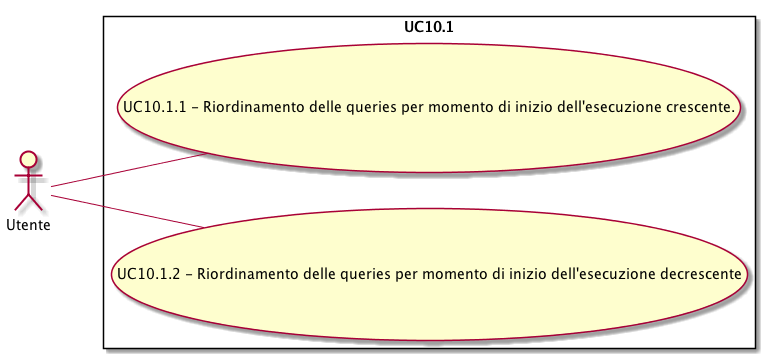
\includegraphics[scale=0.45]{./UC/UC10-1.png}
\caption{Riordinamento delle queries per momento di inizio dell'esecuzione}\label{}
\end{figure}
\begin{itemize}
\item \textbf{Attori}: Utente
\item \textbf{Descrizione}: L'attore vuole riordinare la lista delle queries di una singola trace in base al momento di inizio dell'esecuzione.
\item \textbf{Precondizione}: Deve essere stata visualizzata la lista di queries di una singola trace.
\item \textbf{Flusso principale degli eventi}: L'attore vuole riordinare la lista di queries di una singola trace in base al momento di inizio dell'esecuzione e questo avviene in seguito all'interazione con un componente grafico.
\begin{itemize}
\item Riordinamento delle queries per momento di inizio dell'esecuzione crescente (UC10.1.1)
\item Riordinamento delle queries per momento di inizio dell'esecuzione decrescente (UC10.1.2)
\end{itemize}
\item \textbf{Postcondizione}: La lista di queries di una singola trace viene riordinata in base al momento di inizio dell'esecuzione.
\end{itemize}
\subsection{Caso d'uso UC10.1.1: Riordinamento delle queries per momento di inizio dell'esecuzione crescente}
\begin{itemize}
\item \textbf{Attori}: Utente
\item \textbf{Descrizione}: L'attore vuole riordinare la lista delle queries di una singola trace in base al momento di inizio dell'esecuzione crescente.
\item \textbf{Precondizione}: Deve essere stata visualizzata la lista di queriesdi una singola trace.
\item \textbf{Flusso principale degli eventi}: L'attore vuole riordinare la lista delle queries di una singola trace in base al momento di inizio dell'esecuzione crescente e questo avviene in seguito all'interazione con un componente grafico.
\item \textbf{Postcondizione}: La lista delle queries di una singola trace viene riordinata in base al momento di inizio dell'esecuzione crescente.
\end{itemize}
\subsection{Caso d'uso UC10.1.2: Riordinamento delle queries per momento di inizio dell'esecuzione decrescente}
\begin{itemize}
\item \textbf{Attori}: Utente
\item \textbf{Descrizione}: L'attore vuole riordinare la lista delle queries di una singola trace in base al momento di inizio dell'esecuzione decrescente.
\item \textbf{Precondizione}: Deve essere stata visualizzata la lista di queries di una singola trace.
\item \textbf{Flusso principale degli eventi}: L'attore vuole riordinare la lista delle queries di una singola trace in base al momento di inizio dell'esecuzione decrescente e questo avviene in seguito all'interazione con un componente grafico.
\item \textbf{Postcondizione}: La lista delle queries di una singola trace viene riordinata in base al momento di inizio dell'esecuzione decrescente.
\end{itemize}
\subsection{Caso d'uso UC10.2: Riordinamento delle queries per tempo di esecuzione}
\begin{figure} [H]
\centering
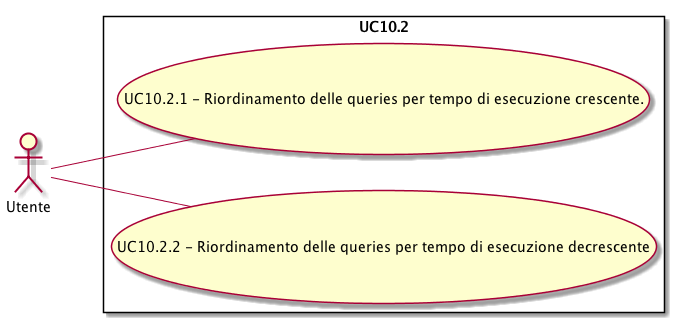
\includegraphics[scale=0.45]{./UC/UC10-2.png}
\caption{Riordinamento delle queries per tempo di esecuzione}\label{}
\end{figure}
\begin{itemize}
\item \textbf{Attori}: Utente
\item \textbf{Descrizione}: L'attore vuole riordinare la lista delle queries di una singola trace in base al tempo di esecuzione.
\item \textbf{Precondizione}: Deve essere stata visualizzata la lista di queries di una singola trace.
\item \textbf{Flusso principale degli eventi}: L'attore vuole riordinare la lista di queries di una singola trace in base al tempo di esecuzione e questo avviene in seguito all'interazione con un componente grafico.
\begin{itemize}
\item Riordinamento delle queries per tempo di esecuzione crescente (UC10.2.1)
\item Riordinamento delle queries per tempo di esecuzione decrescente (UC10.2.2)
\end{itemize}
\item \textbf{Postcondizione}: La lista di queries di una singola trace viene riordinata in base al tempo di esecuzione.
\end{itemize}
\subsection{Caso d'uso UC10.2.1: Riordinamento delle queries per tempo di esecuzione crescente}
\begin{itemize}
\item \textbf{Attori}: Utente
\item \textbf{Descrizione}: L'attore vuole riordinare la lista delle queries di una singola trace in base al tempo di esecuzione crescente.
\item \textbf{Precondizione}: Deve essere stata visualizzata la lista di queries di una singola trace.
\item \textbf{Flusso principale degli eventi}: L'attore vuole riordinare la lista di queries di una singola trace in base al tempo di esecuzione crescente e questo avviene in seguito all'interazione con un componente grafico.
\item \textbf{Postcondizione}: La lista di queries di una singola trace viene riordinata in base al tempo di esecuzione crescente.
\end{itemize}
\subsection{Caso d'uso UC10.2.2: Riordinamento delle queries per tempo di esecuzione decrescente}
\begin{itemize}
\item \textbf{Attori}: Utente
\item \textbf{Descrizione}: L'attore vuole riordinare la lista delle queries di una singola trace in base al tempo di esecuzione decrescente.
\item \textbf{Precondizione}: Deve essere stata visualizzata la lista delle queries di una singola trace.
\item \textbf{Flusso principale degli eventi}: L'attore vuole riordinare la lista di queries di una singola trace in base al tempo di esecuzione decrescente e questo avviene in seguito all'interazione con un componente grafico.
\item \textbf{Postcondizione}: La lista di queries di una singola trace viene riordinata in base al tempo di esecuzione decrescente.
\end{itemize}
\subsection{Caso d'uso UC11: Lettura dei dati da Kibana}
\begin{itemize}
\item \textbf{Attori}: Utente, Kibana
\item \textbf{Descrizione}: Un plugin in seguito ad una richiesta dell'utente reperisce i dati da Kibana
\item \textbf{Precondizione}: Il server di Kibana è avviato e correttamente configurato.
\item \textbf{Flusso principale degli eventi}: L'utente richiede di visualizzare da un plugin dei dati in una forma specifica, dipendente dal tipo di plugin. Tali dati vengono letti da Kibana.
\item \textbf{Postcondizione}: Il plugin riesce a leggere i dati necessari alla visualizzazione da parte dell'utente delle informazioni sull'applicazione monitorata.
\end{itemize}
